\documentclass[11pt,a4paper]{report}
\usepackage[english]{babel}
\usepackage[utf8]{inputenc}
%\usepackage[LFE,LAE]{fontenc}
\usepackage{amsmath}
\usepackage{graphicx}
\usepackage{physics}
\usepackage{float}
\usepackage[margin=1.in]{geometry}
\usepackage{tocloft}
\usepackage{multicol}
\usepackage{hyperref}
\usepackage{rotating}
\usepackage{longtable}
\usepackage{amssymb}
\usepackage[titletoc]{appendix}
\usepackage{setspace}\doublespacing
\usepackage[normalem]{ulem}
\useunder{\uline}{\ul}{}


\usepackage{subcaption} % for adding two figures side by side
\setcounter{secnumdepth}{4}
\setcounter{tocdepth}{4}
\usepackage{enumitem}

\newcommand\tab[1][1cm]{\hspace*{#1}}
\renewcommand{\cfttoctitlefont}{\hfill\Large\bfseries}
\renewcommand{\cftaftertoctitle}{\hfill\hfill}
\renewcommand{\cftloftitlefont}{\hfill\Large\bfseries}
\renewcommand{\cftafterloftitle}{\hfill}
\renewcommand{\cftlottitlefont}{\hfill\Large\bfseries}
\renewcommand{\cftafterlottitle}{\hfill}

% names of supervsior and team
\newcommand{\supervisorname}{\textbf{Dr. FirstName LastName}}

\newcommand{\firststudentname}{\textbf{Student\_FirstName Student\_LastName}}
\newcommand{\firststudentid}{\textbf{42xxxxxxxx}}
\newcommand{\secondstudentname}{\textbf{Student\_FirstName Student\_LastName}}
\newcommand{\secindstudentid}{\textbf{43xxxxxxxx}}


\usepackage{fancyhdr}
 
\pagestyle{fancy}
\fancyhf{}
\fancyhead[LE,RO]{IT Department }
\fancyhead[RE,LO]{Project Documentation Template}
\fancyfoot[CE,CO]{\leftmark}
\fancyfoot[CE,CO]{\thepage}
\renewcommand{\footrulewidth}{0.5pt}

\addto{\captionsenglish}{%
   \renewcommand{\bibname}{References}
}
\addto\captionsenglish{% Replace "english" with the language you use
  \renewcommand{\contentsname}%
    {Table of Contents}%
}
\renewcommand{\cftaftertoctitle}{\hfill}


\usepackage{acro}
\acsetup{first-style=short}
\DeclareAcronym{os}{
  short = OS ,
  long  = Operating System ,
  tag = abbrev
}
\DeclareAcronym{ai}{
  short = AI ,
  long  = Artificial Intelligent ,
  tag = abbrev
}
\DeclareAcronym{dm}{
  short = DM ,
  long  = Data Mining ,
  tag = abbrev
}
\DeclareAcronym{tcp}{
  short = TCP ,
  long  = Transmission Control Protocol ,
  tag = abbrev
}
\DeclareAcronym{ml}{
  short = ML ,
  long  = Machine Learning ,
  tag = abbrev
}
\DeclareAcronym{cnn}{
  short = CNN ,
  long  = Convolutional Neural Network ,
  tag = abbrev
}


\begin{document}

%\setcode{utf8}
\begin{titlepage}
\pagenumbering{gobble}

% header
\begin{center}

\includegraphics[width=\textwidth]{figures/essentials/header.pdf}
\end{center}

\begin{center}
\vspace{3cm}
\huge
\textbf{Project Title}
%%%%%%\textbf{Face Recognition}

\Large
\vspace{3cm}
\textit{Students:}\\
\Large


\begin{tabular}{lr}
{\firststudentname} & {\firststudentid} \\
{\secondstudentname} & {\secindstudentid}
\end{tabular}

\vspace{3cm}
\Large
\textit{Supervisor:}\\
{\supervisorname}

\end{center}
\vfill
\begin{center}	
\textit{A project report submitted in partial fulfillment of the requirements \\
for B.Sc. degree in Information Technology.}
\vspace{5mm}

\textit{Qassim-Saudi Arabia\\
1442/1443 (2020/2021)}

\end{center}
\end{titlepage}
\pagenumbering{gobble}

\pagenumbering{roman}
 \vspace*{2cm}

\begin{center}\section*{Certificate}\end{center}
\addcontentsline{toc}{section}{Certificate}
\begin{spacing}{1.5}
It is certified that project report has been prepared and written under my direct supervision and guidance. The project report is approved for submission for its evaluation.
\end{spacing}
\begin{flushright}
  {\supervisorname}
\end{flushright}

\clearpage
 \vspace*{2cm}

\begin{center}\section*{Dedication}\end{center}
\addcontentsline{toc}{section}{Dedication}
\begin{spacing}{1.5}
It is certified that project report has been prepared and written under my direct supervision and guidance. The project report is approved for submission for its evaluation.
\end{spacing}
\begin{flushright}
{\firststudentname} and {\secondstudentname}
\end{flushright}

\clearpage
 \vspace*{2cm}

\begin{center}\section*{Acknowledgement}\end{center}
\addcontentsline{toc}{section}{Acknowledgement}
\begin{spacing}{1.5}
I would like to thank Mr. A and Mr. B for the efforts that they provided for our team. I would like to thank Mr. A and Mr. B for the efforts that they provided for our team. I would like to thank Mr. A and Mr. B for the efforts that they provided for our team. I would like to thank Mr. A and Mr. B for the efforts that they provided for our team. I would like to thank Mr. A and Mr. B for the efforts that they provided for our team. 
\end{spacing}
\begin{flushright}
{\firststudentname} and {\secondstudentname}
\end{flushright}

\clearpage
 \vspace*{2cm}
\begin{center}\section*{Abstract}\end{center}
\addcontentsline{toc}{section}{Abstract}
\begin{spacing}{1.5}

Abstract Abstract Abstract Abstract Abstract Abstract Abstract Abstract Abstract Abstract Abstract Abstract Abstract Abstract Abstract Abstract Abstract Abstract Abstract Abstract Abstract Abstract Abstract Abstract Abstract Abstract Abstract Abstract Abstract Abstract Abstract Abstract Abstract Abstract Abstract Abstract Abstract Abstract Abstract Abstract Abstract Abstract Abstract Abstract Abstract Abstract Abstract Abstract Abstract Abstract Abstract Abstract Abstract Abstract Abstract Abstract Abstract Abstract Abstract Abstract Abstract Abstract Abstract Abstract Abstract Abstract Abstract Abstract Abstract Abstract Abstract Abstract Abstract Abstract Abstract Abstract Abstract Abstract Abstract Abstract Abstract Abstract Abstract Abstract Abstract Abstract Abstract Abstract Abstract Abstract Abstract Abstract Abstract Abstract Abstract Abstract Abstract Abstract Abstract Abstract Abstract Abstract Abstract Abstract Abstract Abstract Abstract Abstract Abstract Abstract Abstract Abstract Abstract Abstract Abstract Abstract Abstract Abstract Abstract Abstract Abstract Abstract Abstract Abstract Abstract Abstract Abstract Abstract Abstract Abstract Abstract Abstract Abstract Abstract Abstract Abstract Abstract Abstract.\\

{\bf Keywords:} enter, keyword, here.

\end{spacing}
\clearpage

\tableofcontents
\clearpage

\listoffigures
\clearpage

\listoftables
\clearpage
\printacronyms[include=abbrev,name=Abbreviations]
\pagenumbering{gobble}


\pagebreak
\pagenumbering{arabic}
\chapter{INTRODUCTION}
\pagebreak

\begin{center}
{\LARGE\textbf{INTRODUCTION}}
\end{center}

\textcolor{red}{DISCLAIMER: The outline given here is nothing but a suggestion. Please consult your advisor before using them.}

Give an introduction to the report. What is the problem? Why is it important? Did anyone think about it before? All of this should be in brief statements. This is your opportunity to engage the reader in your report. This is also know as the hook.

% ============================================================
\section{Challenges}
\label{sec:challenges}
% ============================================================

What are the challenges of the problem itself. Meaning, if anyone else would try to solve the same problem you are solving, what would be the challenges that they would certainly encounter? Thus the challenges are related to the domain of your project. For example, if your project is about the e-commerce, a challenge could be market penetration. You have to elaborate on each challenge you are aware of and you have to state clearly whether you're addressing the challenge or not. 


% ============================================================
\section{Study Scope}
\label{sec:study_scope}
% ============================================================

Here you'll explain to what extent the research area will be explored, or the boundaries that the research will be performed in. Also, it should be clear what is it that you are NOT doing. For example, a project that is tackling a search algorithm could state that the search is limited to source code (a tool to search for code). Thus, you clearly communicate to the reader that you are not searching the whole web for articles, books, etc. This is just an example, you would have to add as many technical and non-technical boundaries. The clearer you are the less traps are open for the examiners.

% ============================================================
\section{Goals and Objectives}
\label{sec:goals_and_objectives}
% ============================================================

Here you state clearly what are your goals and what should the reader be looking for by the end of reading your report to evaluate your work. These have to be clear statements. However, when you are not sure if you can achieve a goal try to state alternatives (aka mitigations). For example, a goal can be ``by the end of our project we will reduce the search speed by 10\%''. And then elaborate on that goal by for example stating how fast the best tool available now is, etc.

% ============================================================
\section{Report Arrangement}
\label{sec:report_arrangement}
% ============================================================

This section describe briefly how the reset of the report is organized. And most importantly is what should the reader expect from each one. For example, for the literature review, you could say ``we go over all the established work for [project domain]. We also provide extensive background on all the essential technologies we are using in our solution''. This can be a numeric list for each chapter. 
 
\chapter{LITERATURE REVIEW}
\pagebreak

\begin{center}
{\LARGE\textbf{LITERATURE REVIEW}}
\end{center}

\section{Introduction}
Here is an example of one figure introduction introduction introduction introduction introduction introduction introduction introduction introduction introduction introduction introduction introduction introduction introduction introduction introduction introduction introduction introduction introduction introduction introduction introduction introduction introduction introduction introduction introduction introduction introduction introduction introduction introduction introduction introduction introduction introduction introduction introduction introduction introduction introduction introduction introduction introduction introduction introduction introduction introduction introduction introduction introduction introduction introduction introduction introduction introduction introduction introduction introduction introduction introduction introduction as in Figure~\ref{f11}


\begin{figure}[ht]
\begin{center}
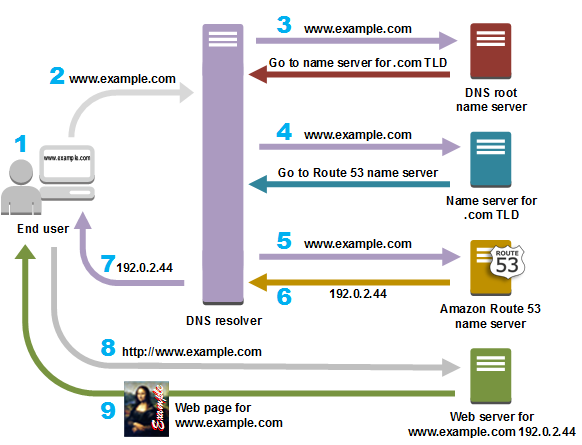
\includegraphics[width=0.6\textwidth]{figures/samples/Fig1.png}
\caption{This is figure 1 in chapter 3}
\label{f11}
\end{center}
\end{figure}

introduction introduction introduction introduction introduction introduction introduction introduction introduction introduction introduction introduction introduction introduction introduction introduction introduction introduction introduction introduction introduction introduction introduction introduction introduction introduction introduction introduction introduction introduction introduction introduction introduction introduction introduction introduction introduction introduction introduction introduction introduction introduction Here is an example of one figure (Figure~\ref{fig:test}) that divided into two sub figures as Figure~\ref{fig:sub1}, Figure~\ref{fig:sub2}, Figure~\ref{fig:sub3}.

\begin{figure}[ht]
\centering
    \begin{subfigure}{.3\textwidth}
         \centering
          
\includegraphics[width=.8\linewidth]{figures/samples/it.png}
           \caption{Machine Learning methods}
        \label{fig:sub1}
        \end{subfigure}%
    \begin{subfigure}{.3\textwidth}
         \centering
        
\includegraphics[width=.8\linewidth]{figures/samples/it.png}
        \caption{Deep learning methods}
        \label{fig:sub2}
        \end{subfigure}
            \begin{subfigure}{.3\textwidth}
         \centering
        
\includegraphics[width=.8\linewidth]{figures/samples/it.png}
        \caption{Recurrent neural networks}
        \label{fig:sub3}
        \end{subfigure}
        \caption{Artificial Intelligent}
\label{fig:test}
\end{figure}

\subsection{Introduction}
Here is an example of one figure
\subsubsection{Introduction}
Here is an example of one figureintroduction introduction introduction introduction introduction introduction introduction introduction introduction introduction introduction introductionintroduction introduction introduction introduction introduction introduction introduction introduction introduction introduction introduction introductionintroduction introduction introduction introduction introduction introduction introduction introduction introduction introduction introduction introductionintroduction introduction introduction introduction introduction introduction introduction introduction introduction introduction introduction introductionintroduction introduction introduction introduction introduction introduction introduction introduction introduction introduction introduction introductionintroduction introduction introduction introduction introduction introduction introduction introduction introduction introduction introduction introductionintroduction introduction introduction introduction introduction introduction introduction introduction introduction introduction introduction introductionintroduction introduction introduction introduction introduction introduction introduction introduction introduction introduction introduction introduction
Here is another example for putting two small figure side by side as in Figure~\ref{fig:test1}, Figure~\ref{fig:test2}.

\begin{figure}[ht]
\centering
\begin{minipage}{.5\textwidth}
  \centering
  
\includegraphics[width=.9\linewidth]{figures/samples/it.png}
  \captionof{figure}{A figure}
  \label{fig:test1}
\end{minipage}%
\begin{minipage}{.5\textwidth}
  \centering
  
\includegraphics[width=.9\linewidth]{figures/samples/it.png}
  \captionof{figure}{Another figure}
  \label{fig:test2}
\end{minipage}
\end{figure}


 introduction introduction introduction introduction ~\cite{ref1} in Figure~\ref{fig1}. introduction introduction introduction introduction introduction introduction introduction introduction introduction introduction introduction introduction introduction introduction introduction introduction introduction ~\cite{ref2}. introduction introduction introduction as in Figure~\ref{fig2} introduction introduction introduction introduction introduction introduction introduction introduction introduction introduction introduction introduction introduction introduction introduction introduction introduction introduction introduction introduction 
~\cite{ref3},\cite{ref4}. 



\begin{figure}[ht]
\begin{center}

\includegraphics[width=0.6\textwidth]{figures/samples/it.png}
\caption{Dummy figure 2}
\label{fig1}
\end{center}
\end{figure}

\begin{sidewaysfigure}[ht]
\begin{center}

\includegraphics[width=0.6\textwidth]{figures/samples/qu.png}
\caption{The image of the introduction}
\label{fig2}
\end{center}
\end{sidewaysfigure}

\hfill \break
\hfill \break
\hfill \break
\hfill \break
\hfill \break
\hfill \break
\hfill \break
\hfill \break
\hfill \break
\hfill \break
\hfill \break
\hfill \break
\hfill \break
\hfill \break
\hfill \break
\hfill \break
\hfill \break

\section{Background}
Introduction introduction introduction introduction introduction introduction introduction introduction introduction introduction introduction introduction introduction introduction introduction introduction introduction introduction introduction introduction introduction introduction introduction introduction introduction introduction introduction introduction introduction introduction \cite{ref1}. 
      

introduction introduction introduction introduction introduction introduction introduction introduction introduction introduction introduction introduction introduction introduction introduction introduction introduction \cite{ref2}. introduction introduction introduction introduction introduction introduction introduction introduction introduction introduction introduction introduction introduction introduction introduction introduction introduction introduction introduction introduction introduction introduction introduction introduction introduction introduction introduction introduction introduction introduction introduction introduction introduction introduction introduction introduction introduction introduction 
\cite{ref5},\cite{ref6}. as shown in eq. (\ref{eq1})

\begin{equation}
Z=\sqrt{X^{2}+Y^{2}}  
\label{eq1}
\end{equation}


Table~\ref{tab1}, Table~\ref{tab2}, Table~\ref{tab3} shows the database for Engineering in different ways


\begin{table}[ht]
\caption{Comparison between related works}
\begin{center}
\begin{tabular}{lllll}
\hline
Name & Method & Ref & Year & Idea                                           \\ \hline

\includegraphics[width=0.2\textwidth, height=30mm]{figures/samples/it.png}   & CNN    & 1   & 2020 &  Dina \\

\includegraphics[width=0.2\textwidth, height=30mm]{figures/samples/it.png}  & RNN    & 2   & 2020 & Mona \\
Dina & CNN    & 1   & 2020 & 
\includegraphics[width=0.2\textwidth, height=20mm]{figures/samples/qu.png} \\
Mona & RNN    & 2   & 2020 &  
\includegraphics[width=0.2\textwidth, height=20mm]{figures/samples/qu.png} \\ \hline
\end{tabular}
    \end{center}
\label{tab1}
\end{table}

\begin{figure}[ht]
\begin{center}

\includegraphics[width=0.1\textwidth]{figures/samples/it.png}
\caption{Dummy figure 2}
\label{fig6}
\end{center}
\end{figure}

\begin{table}[ht]
\caption{Comparison between Wired and wireless networks}
\begin{center}
{\small
%\begin{tabular}{lll}
\begin{tabular}{p{.2\textwidth}p{.2\textwidth}p{.4\textwidth}}

\hline
Specifications       & Wired network    & Wireless network       \\ \hline
Speed of operation   & Higher           & lower compare to wired networks, But advanced wireless technologies such as LTE, LTE-A and WLAN-11ad will make it possible to achieve speed par equivalent to wired network \\
System Bandwidth     & High              & Low, as Frequency Spectrum is very scarse resource    \\
Cost                 & Less as cables are not expensive      & More as wireless subscriber stations, wireless routers, wireless access points and adapters are expensive                 \\
Installation         & Wired network installation is cumbersome and it requires more time   & Wireless network installation is easy and it requires less time             \\
Mobility            & Limited, as it operates in the area covered by connected systems with the wired network                & Not limited, as it operates in the entire wireless network coverage         \\
Transmission medium     & copper wires, optical fiber cables, ethernet   & EM waves or radiowaves or infrared  \\
Network coverage extension    & requires hubs and switches for network coverage limit extension  & More area is covered by wireless base stations which are connected to one another.    \\
Applications           & LAN (Ethernet), MAN        & WLAN, WPAN(Zigbee, bluetooth), Infrared, Cellular(GSM,CDMA, LTE) \\
Channel Interference and signal power loss & Interference is less as one wired network will not affect the other                          & Interference is higher due to obstacles between wireless transmitter and receiver e.g. weather conditions, reflection from walls, etc.                                      \\
QoS (Quality of Service)                   & Better           & Poor due to high value of jitter and delay in connection setup  \\
Reliability           & High compare to wireless counterpart, as manufactured cables have higher performance due to existence of wired technology since years. & Reasonably high, This is due to failure of router will affect the entire network.  \\ \hline
\end{tabular}
}
    \end{center}
\label{tab2}
\end{table}

%\begin{table}[ht]
\begin{sidewaystable}[ht]
\caption{Comparison between Wired and wireless networks}
\begin{center}

\begin{tabular}{p{.2\textwidth}p{.3\textwidth}p{.4\textwidth}}
\hline
Specifications       & Wired network    & Wireless network       \\ \hline
Speed of operation   & Higher           & lower compare to wired networks, But advanced wireless technologies such as LTE, LTE-A and WLAN-11ad will make it possible to achieve speed par equivalent to wired network \\
System Bandwidth     & High              & Low, as Frequency Spectrum is very scarse resource    \\
Cost                 & Less as cables are not expensive      & More as wireless subscriber stations, wireless routers, wireless access points and adapters are expensive                 \\
Installation         & Wired network installation is cumbersome and it requires more time   & Wireless network installation is easy and it requires less time             \\
Mobility            & Limited, as it operates in the area covered by connected systems with the wired network                & Not limited, as it operates in the entire wireless network coverage         \\
Transmission medium     & copper wires, optical fiber cables, ethernet   & EM waves or radiowaves or infrared  \\
Network coverage extension    & requires hubs and switches for network coverage limit extension  & More area is covered by wireless base stations which are connected to one another.    \\
Applications           & LAN (Ethernet), MAN        & WLAN, WPAN(Zigbee, bluetooth), Infrared, Cellular(GSM,CDMA, LTE) \\
Channel Interference and signal power loss & Interference is less as one wired network will not affect the other                          & Interference is higher due to obstacles between wireless transmitter and receiver e.g. weather conditions, reflection from walls, etc.                                      \\
QoS (Quality of Service)                   & Better           & Poor due to high value of jitter and delay in connection setup  \\
Reliability           & High compare to wireless counterpart, as manufactured cables have higher performance due to existence of wired technology since years. & Reasonably high, This is due to failure of router will affect the entire network.    \\ \hline
\end{tabular}

    \end{center}
\label{tab3}
\end{sidewaystable}
%\end{table}

\begin{itemize}     
	\item[$-$] Chapter 1      
	\item[$\square$] Chapter 2     
	 \item Chapter 3       
\end{itemize}

\begin{enumerate}
  \item The labels consists of sequential numbers.
  \item The numbers starts at 1 with every call to the enumerate environment.
\end{enumerate}

\begin{enumerate}
\item The first point
\item the second point
\item the third point
\end{enumerate}

\begin{table}[h]
\caption{Course grades}
\begin{center}
\begin{tabular}{llll}
\hline
Day      & Course Title      & Grade & Level \\ \hline
Saturday & Operating System  & A     & 5     \\ \hline
Sunday   & Data Structure    & B     & 4     \\ \hline
Monday   & Computer Networks & A     & 7     \\ \hline
\end{tabular}
\end{center}
\label{Tab4}
\end{table} 
\chapter{METHODOLOGY}
\pagebreak

\begin{center}
{\LARGE\textbf{METHODOLOGY}}
\end{center}

A research methodology outlines the systematic approach used to collect and analyze data to answer a research question or test a hypothesis. Without any heading, give a simple introduction to what this chapter is about by:
\begin{itemize}
    \item Briefly describe the research question or hypothesis.
    \item Explain why the research is important.
    \item Provide an overview of the research methodology that will be used.
\end{itemize}


\section{Research Design} % (fold)
\label{sec:research_design}

In this section you would focus on the strategy you would follow for conducting your research. 
It is the blueprint for the collection, analysis, and interpretation of data to answer the research questions or test hypotheses.

\begin{itemize}
    \item Determine the type of research design (e.g., experimental, survey, case study). In computer science we rarely use survey based studies as we can usually generate tones of data more reliably and accurately. Thus, if you plan on using a survey, please think about the justification of using it.
    \item Describe your research approach. This refers to the overall plan for the study, which can be quantitative, qualitative, or mixed methods.
    \item [if applicable] Define the target population and sampling method.
    \item [if applicable] describe your sampling method. This refers to the process of selecting participants from a population that is representative of the target population.
\end{itemize}

% section research_design (end)

\section{Data Collection}
\label{sec:data_collection}

Data collection refers to the methods used to collect data, which can be primary or secondary. Primary data collection methods include surveys, interviews, observations, and experiments. Secondary data collection methods include literature review, analysis of existing datasets, and archival research. There are essential steps that you should consider to complete this step.

\begin{itemize}
    \item Conduct pilot tests of data collection instruments.
    \item Collect data from the target population.
    \item Ensure data quality by monitoring data collection and addressing any issues that arise.
\end{itemize}
% section data_collection (end)


\section{Data Analysis}
\label{sec:data_analysis}

The data analysis section refers to the methods used to analyze and interpret the data collected. Quantitative data analysis methods include statistical analysis, while qualitative data analysis methods include content analysis, thematic analysis, and grounded theory analysis.
Here is a list of task that you might think of.

\begin{itemize}
    \item Organize and clean the data.
    \item Choose appropriate statistical or qualitative analysis methods.
    \item Analyze the data and report initial findings.
    \item Consider limitations and potential sources of bias.
\end{itemize}

% section data_analysis (end)


\section{Validation Plan}
\label{sec:validation_plan}

The validation section can describe how you plan to test your work. I.e., what you will need to validate that your solution works. And what would be the measurement of success. 

% section validation_plan (end)


\section{Research Ethics}
\label{sec:research_ethics}

If applicable, the research ethics section should describe the ethical considerations in research, such as informed consent, confidentiality, privacy, and protection of vulnerable populations.

% section research_ethics (end)
 
% \chapter{IMPLEMENTATION AND TESTING}
\pagebreak


\begin{center}
{\LARGE\textbf{IMPLEMENTATION AND TESTING}}
\end{center}

\textcolor{red}{DISCLAIMER: The outline given here is nothing but a suggestion. Please consult your advisor before using them.}

Here you should write a brief introduction to this section. The introduction should not overlap with previous chapters. If there is a need to re-explain something, it should be with a purpose. Your main goal in this 1-2 page intro is to provide a high-level overview of what to expect in this chapter. Also, if you are sharing your code somewhere, you should add the link within this intro.
    
\section{Programming Languages and Tools} % (fold)
\label{sec:programming-languages-and-tools}

Here you should list and explain all programming languages and tools you're using. Whether the tool/language is related to the core functionality of the project or the analysis of the project, it should be added. Avoid saying something like "we use python" it should be more of "for module x we use python because of ..." also, you should add a general statement about the tool/language and its strengths and weaknesses in general.

% section installation (end)

\section{Software Design}% (fold)
\label{sec:software-design}

Start by providing a high-level view of how the system is composed then gradually dive into details. This is a section where lots of diagrams could help. The reader of this section should have a conceptual image of how the system is developed. How many components does the system have and what are they? For each component/module explain what is the main goal of the module and link it to your project's objectives.

The use of widely known diagrams could help you get started. For example, you could use the 4+1 view models to represent your system architecture (\url{https://en.wikipedia.org/wiki/View_model}).

% section programming-languages-and-tools (end)

\section{Algorithm(s)} % (fold)
\label{sec:algorihtms}

Each project should have one or more essential algorithms that are crucial to the project. In this section, you should list them all (if you have more than one) with either pseudocode explaining the algorithm or using the code from one of your programming languages. A pseudocode is preferred as the algorithm is not dependent on a given language but should reflect your code exactly. If someone implements the project using the pseudocode you provided, regardless of the language they use, it should work exactly as your project. 

Please note that you don't just add pseudocode entries here. You are actually explaining it too. Thus, for each algorithm, you should have a pseudocode as a base for your explanation. We expect that you would also provide an explanation of how the algorithm fits within the whole project.

% section algorihtms (end)

\section{Software Testing} % (fold)
\label{sec:software-testing}

For a project to be reliable has to be tested. You're expected to fully or partially test your project. Also, the test could be a module-based test, an integration test, or both (preferred). Whatever you use, you should explain how you established the test cases and provide some test feedback (e.g., test coverage).

Also, the test could be related to some non-functional requirements (e.g., performance or security). If you are targeting one of these non-functional requirements then you should explain how are testing for them.

% section software-testing (end)

\section{Installation} % (fold)
\label{sec:installation}

Think of this section as if you are coming back to this project 10 years from now. Hence, this section should remind you of all the steps/requirements you need to do in order to establish an instance of this project. If you are providing the project as an open-source repo, then it might be enough to explain the high-level details while providing the link here again and making sure that the repo actually has everything one needs to get started.

% section installation (end)


% \chapter{RESULTS AND DISCUSSIONS}
\pagebreak


\begin{center}
{\LARGE\textbf{RESULTS AND DISCUSSIONS}}
\end{center}


\section{Introduction}
Introduction introduction introduction introduction introduction introduction introduction introduction introduction introduction introduction introduction introduction introduction introduction introduction introduction introduction introduction introduction introduction introduction introduction introduction introduction introduction introduction introduction introduction introduction introduction introduction introduction introduction introduction introduction introduction introduction introduction introduction introduction introduction introduction introduction introduction introduction introduction introduction introduction introduction        
% \chapter{CONCLUSIONS AND FUTURE WORK}
\pagebreak

\begin{center}
{\LARGE\textbf{CONCLUSIONS AND FUTURE WORK}}
\end{center}

\textcolor{red}{DISCLAIMER: The outline given here is nothing but a suggestion. Please consult your advisor before using them.}

Very briefly state what this chapter is about. We say very briefly because we all know what conclusion mean. Thus, one paragraph explaining how this chapter is organized might be good enough.


\section{Conclusion} % (fold)
\label{sec:conclusion}

% section conclusion (end)

\subsection{Contributions} % (fold)
\label{sub:contributions}

You should have stated them already in the results sections, but here you briefly re-state you project contributions. You should be as concise and clear as possible. Don't make unrealistic claims. Stay in line with what the result analysis was saying but be enthusiastic about what you made. The statements should be written in a simple paragraph form (1-3 paragraphs is good enough). 

The contribution statements could be of the form ``Through our solutions we were able to reduce x by a factor of y.'' Then elaborate on the statement. Another could be ``A user can accomplish n task in x time which is m times faster than work found in Someone et. al. [1]'' and so on. 

% subsection contributions (end)


\subsection{Limitations} % (fold)
\label{sub:limitations}

Here you do the opposite of what you did in the previous sections. Any project must have some limitations. Actually, when you state the limitations it shows that you have done a thorough analysis of your work and are probably ready to solve them in future work. 

However, not all limitations are solvable. A limitation could be simply a limitation forever. But stating it clearly is good. 

An example of a limitation could be like ``Our system can only process n requests in a second'' you then elaborate on why that is a limitation and why you couldn't overcome it. 

Another example could be ``We only consider x type of inputs.'' And that is fair enough but you should state it clearly and state why you made such a choice.

% subsection limitations (end)

\section{Future Work} % (fold)
\label{sec:future_work}

Projects are always tight on time. You cannot do everything in your mind in a short period of time. Whether that is due to priority or relevance, in this section you state what you would do if you had more time. Future work can be related to a feature you want to add or maybe a type of analysis you wish you could conduct. The more you add the more your project appears to have good potential.

% section future_work (end)



\begin{appendices}
\chapter{Project Installation}
\end{appendices}

\clearpage
\addcontentsline{toc}{chapter}{References}
\bibliographystyle{IEEEtran} % try to use plain or apalike
%https://www.overleaf.com/learn/latex/Bibtex_bibliography_styles
\nocite{*}
 \bibliography{ref.bib}
% change the file name to line up with your bibtex file


\end{document}